\section{Entfernen von Überschneidungen}
\subsection{Beschreibung des Problems}
Wie in Abschnitt \vref{sec:allBet} angedeutet kommt es kommt es bei generierten Graphen zu Überkreuzungen von Teilrouten zwischen jeweils zwei Knoten.
Betrachtet man solche Überkreuzungen im Detail fallen einige Gemeinsamkeiten zwischen ihnen auf.
So ist es beispielsweise immer möglich eine Überkreuzung durch das Verändern der Reihenfolge der Knoten im Pfad aufzulösen und so eine Verringerung in der Gesamtdistanz zu erreichen.

\begin{figure}[h]
    \begin{center}
        \subfloat[Graph mit einer Überkreuzung\label{subfig:graph-with-crossover-and-rect}]{
            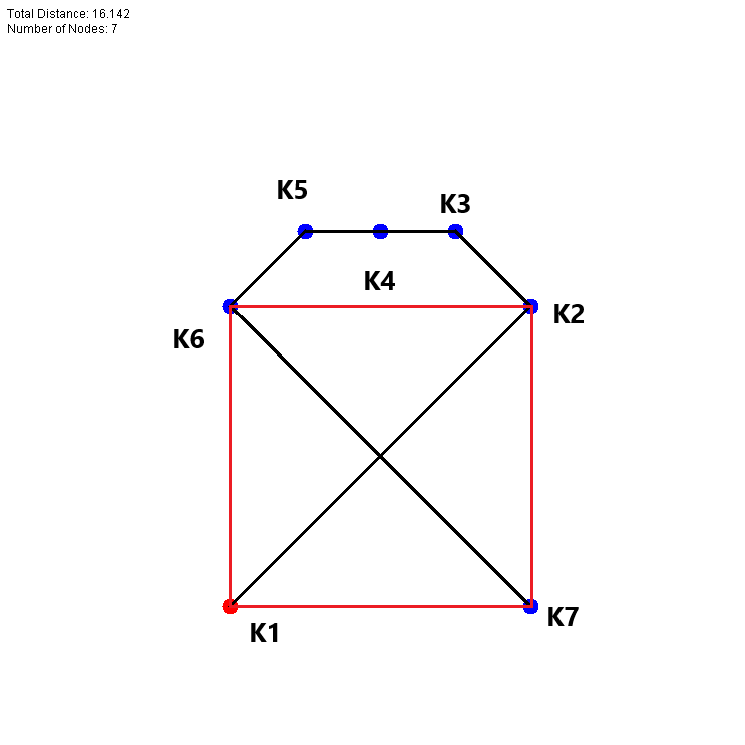
\includegraphics[width=0.35\textwidth]{Bilder/crossover/7_nodes_with_crossover.PNG}
        }
        \hfil
        \subfloat[Aufgelöste Überkreuzung\label{subfig:graph-without-crossover}]{
            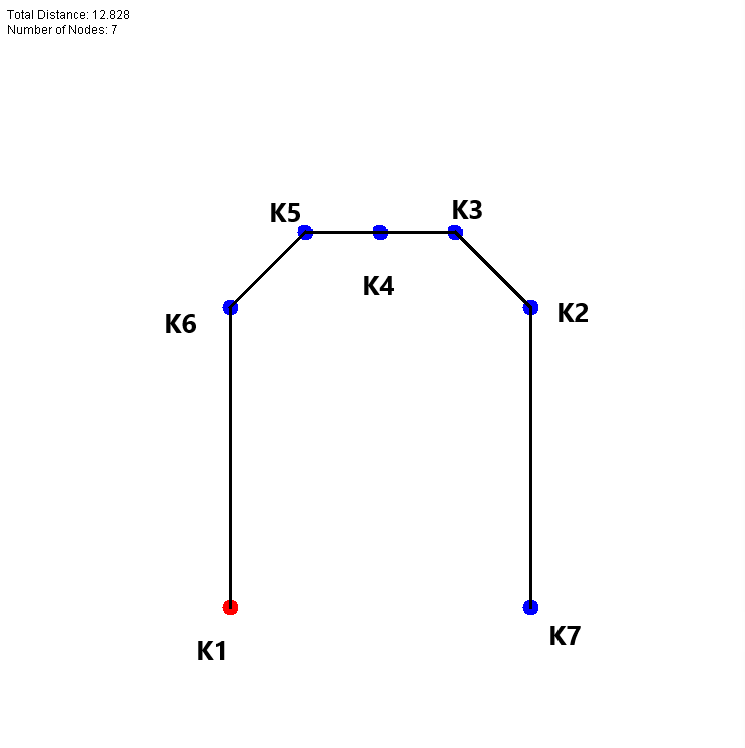
\includegraphics[width=0.35\textwidth]{Bilder/crossover/7_nodes_without_crossover.PNG}
        }
        \caption{Graph mit und ohne Überkreuzung (Das rote Rechteck in Abbildung a) dient späteren Illustrationszwecken)}\label{fig:graph-with-and-without-crossover}
    \end{center}
\end{figure}

Anhand dieses Beispiels wird nun das Entstehen, Erkennen und Auflösen von Überkreuzungen erläutert.

% Allgemein
Eine Überkreuzung repräsentiert das Auftreten eines Schnittpunkts von zwei Kanten eines Graphen in einem für den Graphen relevanten Bereich.
Ein Schnittpunkt von zwei Kanten bedeutet hier, dass keine der vier Knoten gleich sein dürfen.
Besteht eine Überkreuzung also aus den Knotenpaaren $A$ und $B$ mit $A=K_{A_1},K_{A_2}$ und $B=K_{B_1},K_{B_2}$, dann muss gelten $K_{A_1} \neq K_{A_2} \neq K_{B_1} \neq K_{B_2}$.
Ist diese Bedingung nicht erfüllt, kann es keine Überkreuzung geben.
Sind nur drei der vier benötigten Knoten einzigartig kann es nicht zu einer Überkreuzung kommen, da dies einen zusammenhängenden Streckenabschnitt der Form $K_1, K_2, K_3$ darstellen würde.

\subsection{Erkennnen von Überkreuzungen}
Um Überkreuzungen erkennen zu können ist die Bedingung \enquote{in einem für den Graphen relevanten Bereich} wichtig.
Betrachtet man zwei zufällig ausgewählte Kanten als unendliche Linien, stellt man sie also in der zweidimensionalen Ebene als lineare Funktion, mit einer Steigung und einem Schnittpunkt mit der Ordinate, dar, dann schneiden sich alle diese Funktionen an irgendeinem Punkt, es sei denn sie sind parallel zueinander.
Um zu überprüfen, ob eine Überkreuzung im für die Generierung eines Graphen relevanten Bereich ist, wird zuerst der Schnittpunkt der beiden Kanten berechnet.
Dazu wird aus zwei Knoten einer Kante eine lineare Funktion der Form $f(x) =mx+n$ simuliert, wobei $m=\frac{\Delta y}{\Delta x}$ und $n=y - mx$.
Sind die Knoten der beiden Kanten nun $A_1,A_2$ und $B_1,B_2$, dann ergibt sich für die Berechnung der Schnittstelle:
\begin{equation}
    \label{eq:calculation-xs}
    % x_S = (y_{B_1} - (x_{B_1}\cdot \frac{(y_{A_2} - y_{A_1})}{(x_{A_2} - xy_{A_1})}))
    x_S = \frac{(y_{B_1} - \frac{y_{B_2} - y_{B_1}}{x_{B_2} - x_{B_1}}\cdot x_{B_1}) - (y_{A_1} - \frac{y_{A_2} - y_{A_1}}{x_{A_2} - x_{A_1}}\cdot x_{A_1})}{(\frac{y_{A_2} - y_{A_1}}{x_{A_2} - x_{A_1}}) - (\frac{y_{B_2} - y_{B_1}}{x_{B_2} - x_{B_1}})} 
\end{equation}
\begin{equation}
    \label{eq:calculation-ys}
    y_S = \frac{y_{A_2} - y_{A_1}}{x_{A_2} - x_{A_1}}\cdot x_S + (y_{A_1} - \frac{y_{A_2} - y_{A_1}}{x_{A_2} - x_{A_1}}\cdot x_{A_1})
\end{equation}
Mit $x_S$ und $y_S$ lässt sich der Punkt $S(x_S|y_S)$ konstruieren.
\\\\
Mit Hilfe des Punkts $S$ gilt es nun zu überprüfen, ob sich dieser im relevanten Bereich befindet.
Um dies zu bestimmen wird um die Knoten beider Kanten jeweils ein Recht simuliert, wie es beispielhaft in Abbildung \vref{subfig:graph-with-crossover-and-rect} eingezeichnet ist.
Eine Überkreuzung ist genau dann für den Algorithmus relevant, wenn sie in den Rechtecken beider Kanten liegt.
Um dies zu überprüfen wird folgender Algorithmus angewandt:
\begin{algorithm}[H]
    \caption{Erkennen von Überkreuzungen}
    \label{alg:check-point-in-rect}
    \begin{algorithmic}[1]
        \Require Knoten $A_1,A_2$, Punkt $P$
        \State score $\gets 0$
        \If{$x_{A_1} > x_{A_2}$}
            \If{$x_P > x_{A_2}$ \textbf{and} $x_P < x_{A_1}$}
                \State score $\gets$ score $+ 1$
            \EndIf
        \Else
            \If{$x_P < x_{A_2}$ \textbf{and} $x_P > x_{A_1}$}
                \State score $\gets$ score $+ 1$
            \EndIf
        \EndIf

        \If{$y_{A_1} > y_{A_2}$}
            \If{$y_P < y_{A_1}$ \textbf{and} $y_P > y_{A_2}$}
                \State score $\gets$ score $+ 1$
            \EndIf
        \Else
            \If{$y_P > y_{A_1}$ \textbf{and} $y_P < y_{A_2}$}
                \State score $\gets$ score $+ 1$
            \EndIf
        \EndIf\\
        \Return (score $== 2$)
        \Comment score $==2$ gibt wahr zurück und signalisiert, dass $P$ im Rechteck von $A_1$ und $A_2$ ist
    \end{algorithmic}
\end{algorithm}
An dieser Stelle sei angemerkt, dass das Problem der Überkreuzungserkennung auch mit Hilfe von Vektorenskalierung lösbar ist.
Dieses Verfahren wird jedoch in dieser Arbeit nicht diskutiert.


\subsection{Auflösen von Überkreuzungen}

Um einen Algorithmus zur Auflösung von Überkreuzungen entwickeln zu können, ist es wichtig die Knoten um eine Überkreuzung herum vor und nach deren Auflösung zu betrachten.
Dazu kann als Beispiel wieder Abbildung \vref{fig:graph-with-and-without-crossover} dienen.
Reihenfolge der Knoten in Abbildung \vref{subfig:graph-with-crossover-and-rect} ist $$P_{alt} = K_1, K_2, K_3, K_4, K_5, K_6, K_7$$
Die Reihenfolge der Knoten nach dem Auflösen in Abbildung \vref{subfig:graph-without-crossover} ist $$P_{neu} = K_1, K_6, K_5, K_4, K_3, K_2, K_7$$
In diesem Beispiel seien die betroffenen Kanten $A$ und $B$ mit den Knoten $A_1 = K_1$, $A_2 = K_2$ und $B_1 = K_6$, $B_2 = K_7$.
Die hier interessanten Knoten sind $K_2$ bis $K_6$, da sich deren Reihenfolge umkehrt.
Daraus kann gefolgert werden, dass zum Auflösen einer Überkreuzung das Umkehren der betroffenen Knoten in der Mitte reicht.
Diese betroffenen Knoten bestimmen sich durch die Kanten $A$ und $B$ -- der erste umzukehrende Knoten ist immer $A_2$, während der letzte $B_1$ ist.
Dies ist allerdings nur unter der Bedingung wahr, dass $A$ im Graph vor $B$ ist.
% Ist dies nicht der Fall müssen $A$ und $B$ getauscht werden, sodass 
Ist dies nicht der Fall kehren sich die Rollen der Knoten um und $B_1$ ist der erste, während $A_2$ der letzte umzukehrende Knoten ist.
Ein Algorithmus, der auf einem Pfad mit Überkreuzung und bekannten $A$ und $B$ eben dieses Tauschen ausführt, findet sich im Anhang unter Algorithmus \vref{alg:swap-nodes-inbetween}.
\\\\
% Ein vollständiger Algorithmus, der die aufgeführten Methodiken anwendet um Überkreuzungen zu erkennen und aufzulösen könnte beispielhaft
Ein vollständiger Algorithmus, der die aufgeführten Methodiken anwenden soll, um Überkreuzungen zu erkennen und aufzulösen, müssen also alle Kanten gegeneinander geprüft werden.
Eine simple Umsetzung davon, die alle beschriebenen Methodiken mit einschließt kann sein
\begin{algorithm}
    \caption{Erkennen und Auflösen von Überkreuzungen auf einem Pfad}
    \label{alg:handle-crossover}
    \begin{algorithmic}[1]
        \Require Pfad $P$
        \Require $P=p_1,p_2\cdots,p_n$, $n \geq 4$, $\forall p \in G$
        
        \For{$a \gets 2$, $a \leq n$, $a \gets a + 1$}
            \For{$b \gets b$, $b \leq n$, $b \gets b + 1$}
                \If{\textbf{not} ($p_a \neq p_{b} \textrm{\textbf{ and }} p_a \neq p_{b-1} \textrm{\textbf{ and }} p_{a-1} \neq p_b \textrm{\textbf{ and }} p_{a-1} \neq p_{b-1}$}
                    \State \textsc{continue}
                \EndIf
                \State $x_S \gets $ nach \vref{eq:calculation-xs}
                \Comment $p_a$ und $p_{a-1}$ entsprechen $A_1$ und $A_2$ 
                \State $y_S \gets $ nach \vref{eq:calculation-ys}
                \Comment $p_b$ und $p_{b-1}$ entsprechen $B_1$ und $B_2$ 
                \If{\textsc{check}($p_a,p_{a-1},S(x_S|y_S)$) \textbf{and} \textsc{check}($p_b,p_{b-1},S(x_S|y_S)$)} 
                \Comment \textsc{check} repräsentiert dabei \ac{Alg.} \vref{alg:check-point-in-rect}
                    \State $P \gets $ \textsc{resolve}($P$, $p_a$, $p_{b-1}$)
                    \Comment Auflösen der Überkreuzung mit \ac{Alg.} \vref{alg:swap-nodes-inbetween}
                \EndIf
            \EndFor
        \EndFor
    \end{algorithmic}
\end{algorithm}

Wird das Entfernen von Überkreuzungen nach diesem Prinzip implementiert, ergeben sich einige Randbedingungen, die es Wert sind erwähnt zu werden.
Aufgrund der geschachtelten Iterationen über die Kanten des Graphs lässt sich eine Zeitkomplexität von $$O(n) = n^2$$ ermitteln, womit der Algorithmus im Rahmen der polynomialen Zeitkomplexitätsklasse liegt. 
Dies bedeutet, dass die Laufzeit des Algorithmus proportional zum Quadrat seiner Eingabemenge wächst.\autocite[15]{Gurski.2010}
Als Eingabemenge können hier Knoten bzw. Kanten eines Graphen behandelt werden, wobei $n$ die Menge der Knoten repräsentiert.
\\
Ein Algorithmus, der Überkreuzungen aus einem Graph entfernt, arbeitet also mit einer ähnlichen Laufzeit wie die Heuristiken, die den Graph vorher erzeugen.
\\\\
Weiterhin ist es möglich, dass durch das Auflösen einer Überkreuzung eine weitere, neue entsteht.
Falls dies so geschieht, dass in den restlichen Iterationen über die Kanten diese Überkreuzung nicht mehr erkannt wird, beispielsweise, wenn dies in der letzten Iteration passiert, dann wird die Überkreuzung nicht vom Algorithmus aufgelöst.
Eine Möglichkeit dies zu umgehen ist durch das rekursive Aufrufen des Algorithmus, damit mehrmals auf Überkreuzungen überprüft wird.
Allerdings besteht hier Bedarf eine solche Implementierung genauer zu untersuchen, was in dieser Arbeit nicht behandelt wird.
